\begin{figure}[H]
    \centering       
\tikzset{every picture/.style={line width=0.75pt}} %set default line width to 0.75pt        

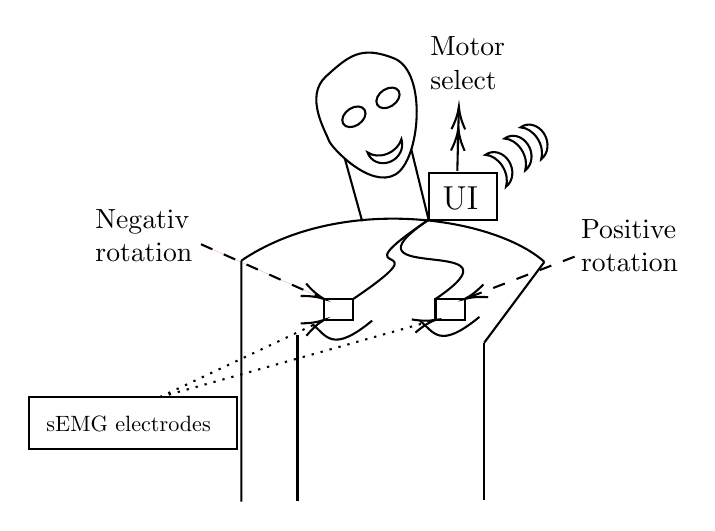
\begin{tikzpicture}[x=0.75pt,y=0.75pt,yscale=-1,xscale=1]
%uncomment if require: \path (0,348.6666564941406); %set diagram left start at 0, and has height of 348.6666564941406

%Straight Lines [id:da48983191890161915] 
\draw    (302.93,184.24) -- (302.95,300.29) ;


%Straight Lines [id:da551487490016626] 
\draw    (330,220) -- (330,300) ;


%Straight Lines [id:da6135134184778834] 
\draw    (419.95,223.79) -- (419.95,299.79) ;


%Curve Lines [id:da40002913632145076] 
\draw    (337.25,214.92) .. controls (344.01,220.3) and (346.39,229.26) .. (365.97,213.14) ;


%Curve Lines [id:da017442708579094912] 
\draw    (388.93,213.13) .. controls (395.68,218.5) and (398.07,227.47) .. (417.65,211.35) ;


%Shape: Rectangle [id:dp2948369463848257] 
\draw   (342.82,202.73) -- (356.83,202.73) -- (356.83,212.78) -- (342.82,212.78) -- cycle ;
%Shape: Rectangle [id:dp8177370839769769] 
\draw   (396.48,202.73) -- (410.49,202.73) -- (410.49,212.78) -- (396.48,212.78) -- cycle ;
%Shape: Polygon Curved [id:ds39308421777793057] 
\draw   (343.78,95.42) .. controls (354.51,85.74) and (360.48,80.36) .. (376.58,86.82) .. controls (392.67,93.27) and (389.17,135.74) .. (377.17,142.74) .. controls (365.18,149.74) and (346.17,129.83) .. (344.97,126.07) .. controls (343.78,122.31) and (333.05,105.1) .. (343.78,95.42) -- cycle ;
%Curve Lines [id:da9166271647364232] 
\draw    (302.93,184.24) .. controls (350.63,151.98) and (424.5,162.97) .. (448.95,184.83) ;


%Straight Lines [id:da6940855715795691] 
\draw    (352.82,135.14) -- (361.17,165.25) ;


%Straight Lines [id:da06557587996091874] 
\draw    (384.85,130.69) -- (393.16,164.56) ;


%Shape: Rectangle [id:dp44542314487649004] 
\draw   (393.16,141.97) -- (426.16,141.97) -- (426.16,164.56) -- (393.16,164.56) -- cycle ;
%Straight Lines [id:da5886591469978335] 
\draw    (448.95,184.83) -- (419.95,223.79) ;


%Curve Lines [id:da438028737656337] 
\draw    (356.83,202.73) .. controls (404.53,170.47) and (345.46,196.83) .. (393.16,164.56) ;


%Curve Lines [id:da298231790072667] 
\draw    (396.48,202.73) .. controls (444.18,170.47) and (345.46,196.83) .. (393.16,164.56) ;


%Straight Lines [id:da17698811288515226] 
\draw  [dash pattern={on 0.84pt off 2.51pt}]  (263.68,250.01) -- (341.01,213.63) ;
\draw [shift={(342.82,212.78)}, rotate = 514.81] [color={rgb, 255:red, 0; green, 0; blue, 0 }  ][line width=0.75]    (10.93,-3.29) .. controls (6.95,-1.4) and (3.31,-0.3) .. (0,0) .. controls (3.31,0.3) and (6.95,1.4) .. (10.93,3.29)   ;

%Straight Lines [id:da4704201066732616] 
\draw  [dash pattern={on 0.84pt off 2.51pt}]  (263.68,250.01) -- (394.55,213.32) ;
\draw [shift={(396.48,212.78)}, rotate = 524.3399999999999] [color={rgb, 255:red, 0; green, 0; blue, 0 }  ][line width=0.75]    (10.93,-3.29) .. controls (6.95,-1.4) and (3.31,-0.3) .. (0,0) .. controls (3.31,0.3) and (6.95,1.4) .. (10.93,3.29)   ;

%Shape: Rectangle [id:dp09154428052258479] 
\draw   (200.5,249.85) -- (300.86,249.85) -- (300.86,274.77) -- (200.5,274.77) -- cycle ;
%Shape: Moon [id:dp8725784672937908] 
\draw   (420.51,133.29) .. controls (423.99,130.68) and (429.04,131.98) .. (431.79,136.21) .. controls (434.54,140.43) and (433.95,145.98) .. (430.48,148.6) .. controls (431.36,145.65) and (430.77,141.85) .. (428.64,138.58) .. controls (426.51,135.31) and (423.39,133.4) .. (420.51,133.29) -- cycle ;
%Shape: Moon [id:dp39582079060737096] 
\draw   (429.75,125.43) .. controls (433.23,122.81) and (438.27,124.11) .. (441.03,128.34) .. controls (443.78,132.56) and (443.19,138.11) .. (439.71,140.73) .. controls (440.6,137.79) and (440.01,133.98) .. (437.88,130.71) .. controls (435.75,127.44) and (432.63,125.54) .. (429.75,125.43) -- cycle ;
%Shape: Moon [id:dp049975679573210696] 
\draw   (437.45,120.04) .. controls (440.92,117.42) and (445.97,118.73) .. (448.72,122.95) .. controls (451.48,127.18) and (450.89,132.73) .. (447.41,135.35) .. controls (448.3,132.4) and (447.71,128.59) .. (445.58,125.33) .. controls (443.45,122.06) and (440.33,120.15) .. (437.45,120.04) -- cycle ;
%Shape: Moon [id:dp9195347803104288] 
\draw   (380.06,125.7) .. controls (381.51,129.99) and (379.03,134.9) .. (374.53,136.66) .. controls (370.02,138.43) and (365.19,136.38) .. (363.74,132.09) .. controls (366.15,133.77) and (369.73,134.14) .. (373.21,132.78) .. controls (376.7,131.41) and (379.22,128.66) .. (380.06,125.7) -- cycle ;
%Shape: Ellipse [id:dp8827523909159829] 
\draw   (362.38,111.69) .. controls (363.5,113.77) and (362.07,116.91) .. (359.19,118.7) .. controls (356.31,120.49) and (353.06,120.25) .. (351.95,118.17) .. controls (350.83,116.09) and (352.27,112.96) .. (355.15,111.17) .. controls (358.03,109.38) and (361.27,109.61) .. (362.38,111.69) -- cycle ;
%Shape: Ellipse [id:dp42511842093367047] 
\draw   (378.81,102.58) .. controls (379.92,104.66) and (378.49,107.79) .. (375.61,109.58) .. controls (372.73,111.38) and (369.49,111.14) .. (368.37,109.06) .. controls (367.26,106.98) and (368.69,103.85) .. (371.57,102.06) .. controls (374.45,100.27) and (377.69,100.5) .. (378.81,102.58) -- cycle ;
%Straight Lines [id:da8820566539783692] 
\draw    (407,141) -- (407.45,122.33) ;
\draw [shift={(407.5,120.33)}, rotate = 451.39] [color={rgb, 255:red, 0; green, 0; blue, 0 }  ][line width=0.75]    (10.93,-3.29) .. controls (6.95,-1.4) and (3.31,-0.3) .. (0,0) .. controls (3.31,0.3) and (6.95,1.4) .. (10.93,3.29)   ;

%Straight Lines [id:da5478933045813028] 
\draw    (407.25,130.67) -- (407.7,112) ;
\draw [shift={(407.75,110)}, rotate = 451.39] [color={rgb, 255:red, 0; green, 0; blue, 0 }  ][line width=0.75]    (10.93,-3.29) .. controls (6.95,-1.4) and (3.31,-0.3) .. (0,0) .. controls (3.31,0.3) and (6.95,1.4) .. (10.93,3.29)   ;

%Straight Lines [id:da9326088231862386] 
\draw [fill={rgb, 255:red, 216; green, 21; blue, 21 }  ,fill opacity=1 ] [dash pattern={on 4.5pt off 4.5pt}]  (283.5,176.33) -- (340.99,201.92) ;
\draw [shift={(342.82,202.73)}, rotate = 203.99] [color={rgb, 255:red, 0; green, 0; blue, 0 }  ][line width=0.75]    (10.93,-3.29) .. controls (6.95,-1.4) and (3.31,-0.3) .. (0,0) .. controls (3.31,0.3) and (6.95,1.4) .. (10.93,3.29)   ;

%Straight Lines [id:da06992380639248452] 
\draw  [dash pattern={on 4.5pt off 4.5pt}]  (463.5,182.33) -- (412.36,202.01) ;
\draw [shift={(410.49,202.73)}, rotate = 338.95] [color={rgb, 255:red, 0; green, 0; blue, 0 }  ][line width=0.75]    (10.93,-3.29) .. controls (6.95,-1.4) and (3.31,-0.3) .. (0,0) .. controls (3.31,0.3) and (6.95,1.4) .. (10.93,3.29)   ;


% Text Node
\draw (408.49,154.29) node  [align=left] {{\large UI}};
% Text Node
\draw (248.65,262.63) node [scale=0.8] [align=left] {sEMG electrodes};
% Text Node
\draw (412,89) node  [align=left] {Motor\\select};
% Text Node
\draw (256,172) node  [align=left] {Negativ\\rotation};
% Text Node
\draw (490,177) node  [align=left] {Positive\\rotation};


\end{tikzpicture}


   \caption{Physical setup of control}
    \label{fig:PCS}
\end{figure}

